\documentclass[12pt]{article}
\usepackage{xeCJK}
\usepackage{amsmath}
\usepackage{pdfpages}
\usepackage[colorlinks,linkcolor=red]{hyperref}

\title{Project 1}
\author{
李林翼 \footnote{计43, 2014011361, limyik.li96@gmail.com}
\ 朱祺 \footnote{计43, 2014011336, zhu-q14@mails.tsinghua.edu.cn}
}
\begin{document}
\maketitle{}
\tableofcontents
\newpage

\section{数据预处理和可视化}
\subsection{新闻数据读入与建立数据框对象}
第一步是数据的读取。此处为了后面便于处理,将读取的数据持久化,保存为 result/data.csv 文件。
可以分为以下三步:确定要读取的新闻的属性;读取新闻到data.frame;保存为 .csv 文件。
\subsubsection{确定要读取的新闻的属性}
根据proj1的要求和new\_york\_times\_annotated\_corpus.pdf文件,选定以下属性读取:
\begin{description}
  \item[docid]
  新闻唯一标识符,也是文档的名字
  \item[title]
  新闻的标题
  \item[categories]
  新闻的类别,使用online\_sections属性。例子:``Business; Technology''。
  \item[locations]
  新闻中提到的地点,使用Locations和Online\_Locations属性。例子:``NEW YORK, NY''。
  \item[day\_of\_month,month,year]
  发行日期,使用publication\_*属性。例子:26; 06; 1995。
  \item[publication\_date]
  发行日期,使用Publication Date属性。例子:19950627T000000。
  \item[body]
  新闻正文。
\end{description}
\subsubsection{读取新闻到data.frame}
这一部分主要的函数readDoc()在readDoc.R中。使用了XML和stringr两个库辅助处理。
属性不存在时标记为NA。
\subsubsection{数据持久化}
主要的函数readAll()和extractAll()在readDoc.R中。读取目录下所有新闻,将data.frame写入
data.csv

\subsection{对新闻全文进行预处理}
tm库中有很方便的函数可以进行预处理,包括去除标点符号、停用词、数字、空白字符,将
大写字母都转化为小写,以及词干化处理。所有的这些处理都可以使用tm\_map()函数,
通过map的方式将转化函数应用到每一个文档语料上。主要函数getCorpus()在process.R中,返回Corpus。
\subsection{将新闻表示成BagOfWords向量}
利用上一步得到的Corpus,借助DocumentTermMatrix函数,可以得到文档-词条矩阵,
每一行即是BagOfWords向量。
\subsection{筛选出出现次数大于100的词并画 wordcloud}
DocumentTermMatrix得到的文档-词条矩阵通过findFreqTerms函数找出出现次数大于100的词。
单词-频数表保存在result/wordFrequency.csv中。利用wordcloud函数绘制云图。
实现在process.R的drawWordCloud()中。结果见\ref{fig:wordCloud}。
\begin{figure}[htbp]
\centering
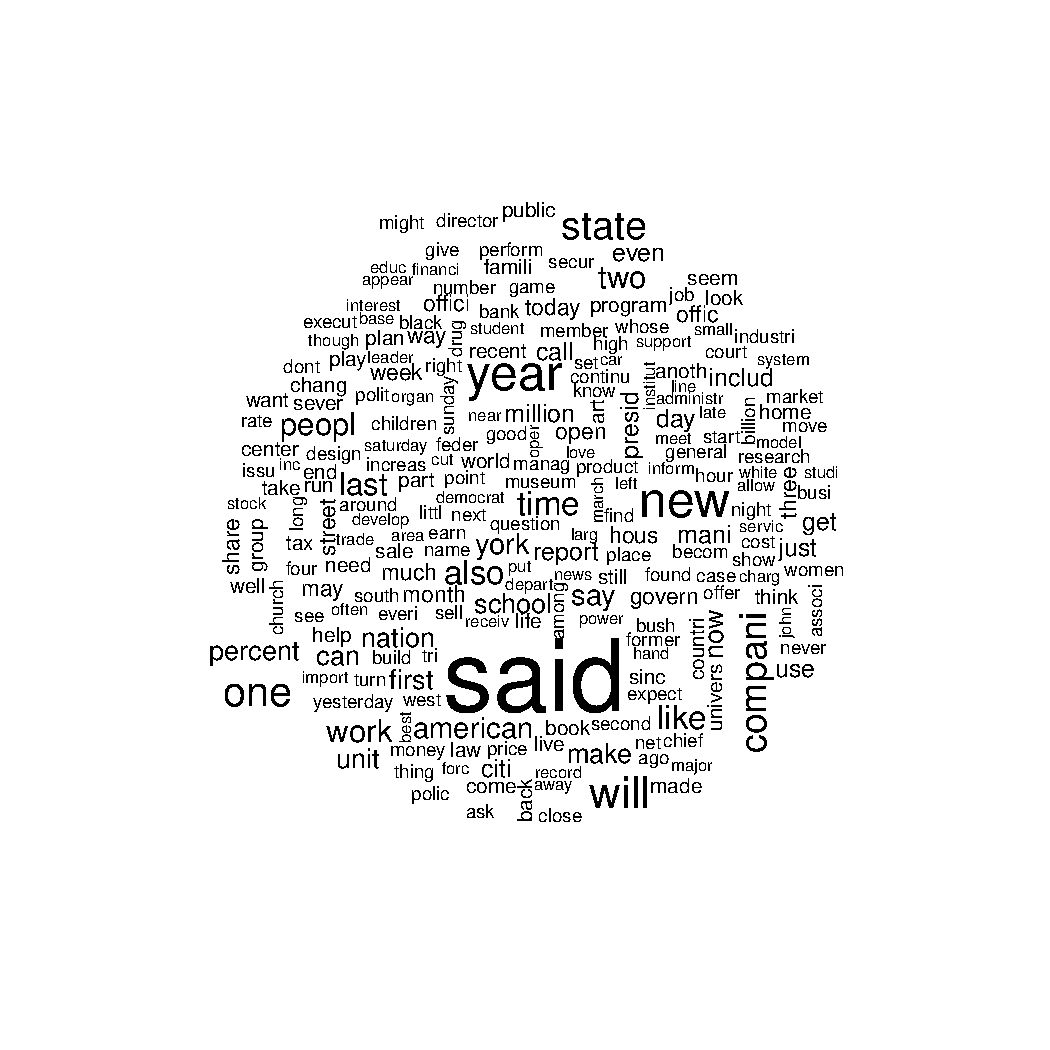
\includegraphics[width=1.0\textwidth]{../result/wordCloud.pdf}
\caption{wordCloud}
\label{fig:wordCloud}
\end{figure}
出现最多的词是said,挺符合新闻报道的特点的。其他高频词如state、compani、school、work、peopl、
american还是很合理的。但也有些没什么实际含义的词如also、dont、next、get、just。

\subsection{画出单词长度的分布直方图}
与上类似,findFreqTerms(DocumentTermMatrix(corpus), 0)得到所有word,按单词长度统计。
利用ggplot2中qplot画图。实现在process.R的drawWordLength()中。结果见\ref{fig:wordLength}。
\begin{figure}[htbp]
\centering
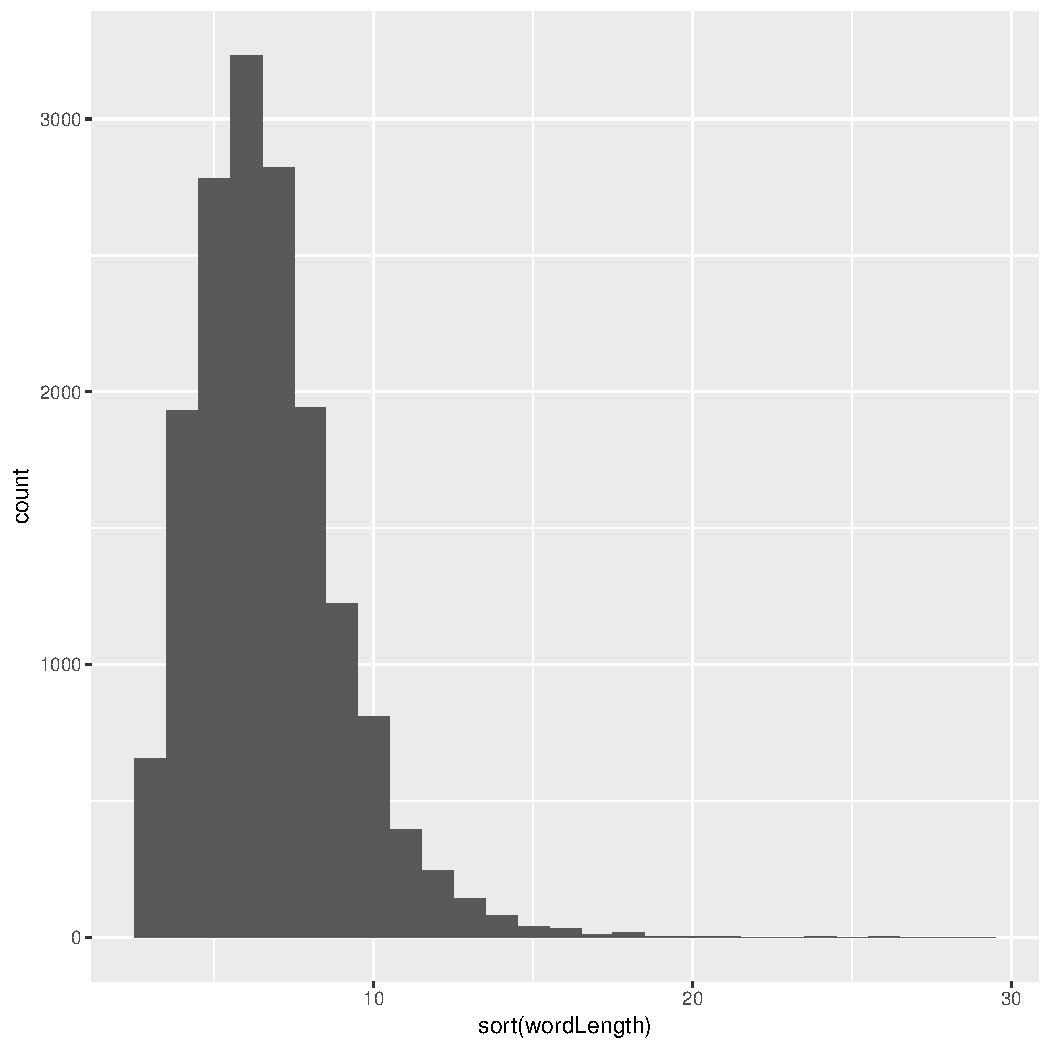
\includegraphics[width=1.0\textwidth]{../result/wordLength.pdf}
\caption{wordLength}
\label{fig:wordLength}
\end{figure}
可以看到单词的长度基本上在10以内,主要集中在3-6个字母之间。

\subsection{画出新闻类别的分布直方图}
将新闻按照类别进行统计。每个新闻可能有多个类别,要在这些类别下都计数。实现在process.R的
drawCategories()中。利用ggplot()画图,
结果见\ref{fig:categories}。最多的是business, new york, region,其他的如art, sports, 
opinions也不少,偏向生活的类别含有的新闻比较少,如theater, travel, dining, automobile。
\begin{figure}[htbp]
\centering
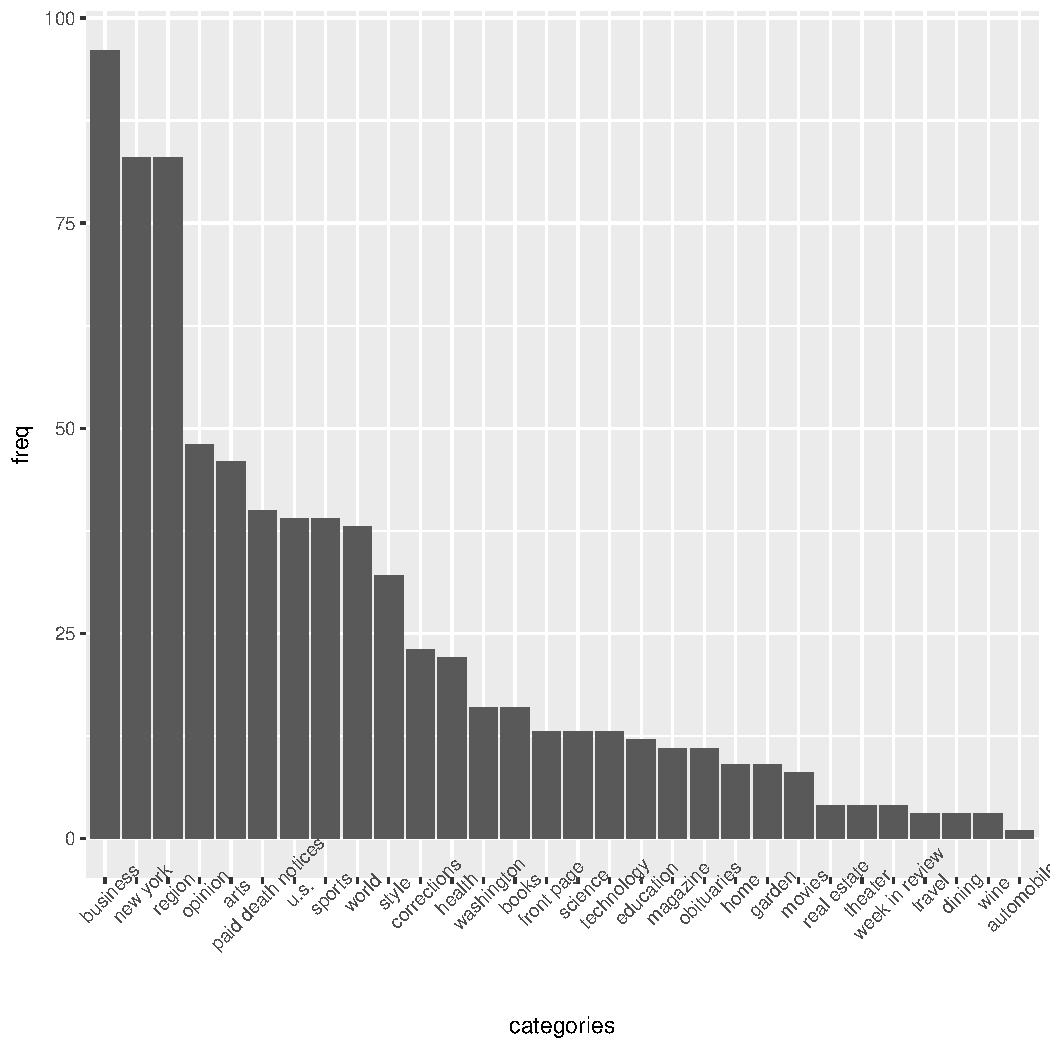
\includegraphics[width=1.0\textwidth]{../result/categories.pdf}
\caption{categories}
\label{fig:categories}
\end{figure}

\subsection{画出每个月新闻数量的分布直方图}
按月绘制新闻的出版数量,从所有新闻中找出最早的出版月份作为第0个月,其他出版月份以此为参照递推,次年1
月为第13个月。实现在process.R的drawTimeLine()中。利用ggplot()画图,结果见
\ref{fig:timeLine}。

\begin{figure}[htbp]
\centering
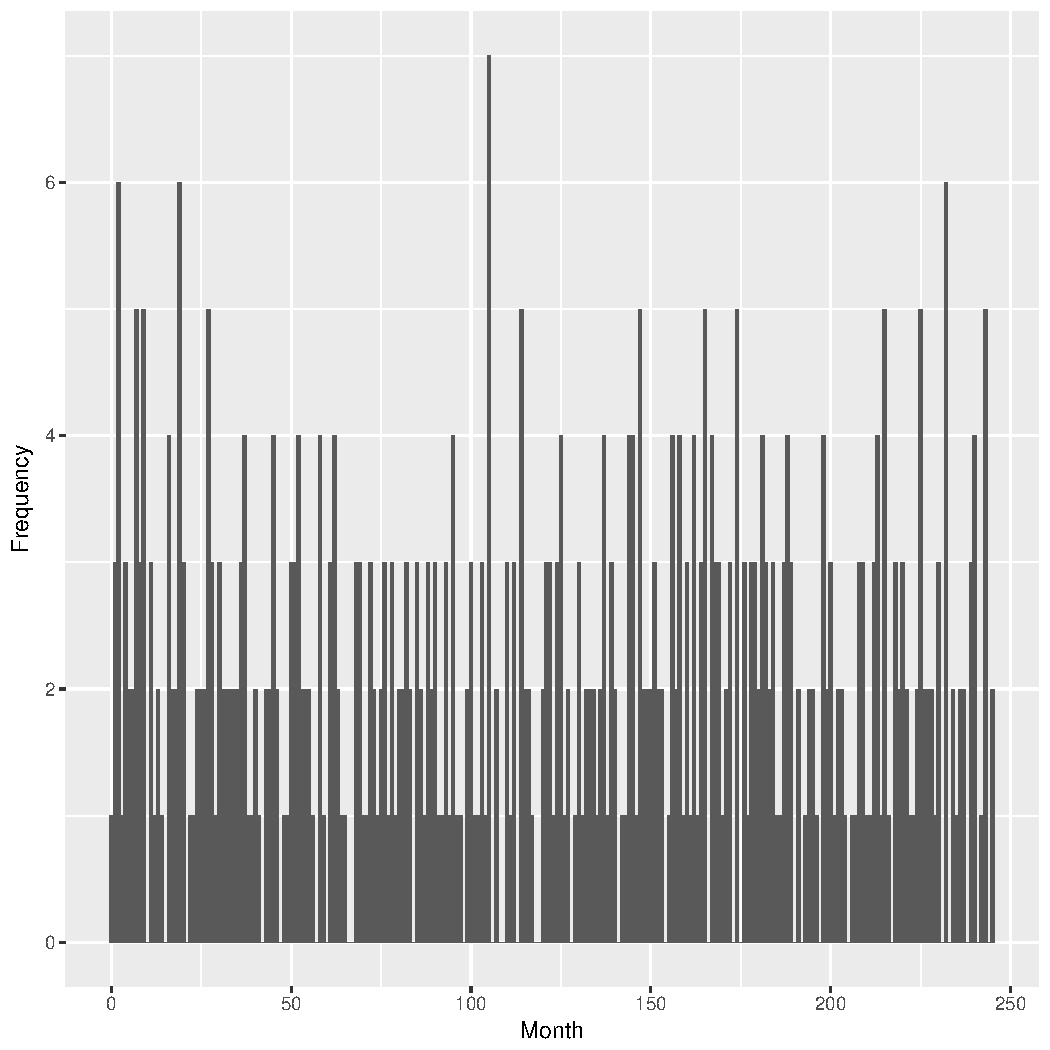
\includegraphics[width=1.0\textwidth]{../result/timeLine.pdf}
\caption{timeLine}
\label{fig:timeLine}
\end{figure}

\subsection{画出每年新闻数量的分布直方图}
由于每个月新闻数量的分布直方图太过密集,于是稍微修改drawTimeLine()函数得到drawTimeLineYear()
函数,用于画出每年新闻数量的分布直方图。见\ref{fig:timeLineYear}。可以看出都在20上下,波动不大。
\begin{figure}[htbp]
\centering
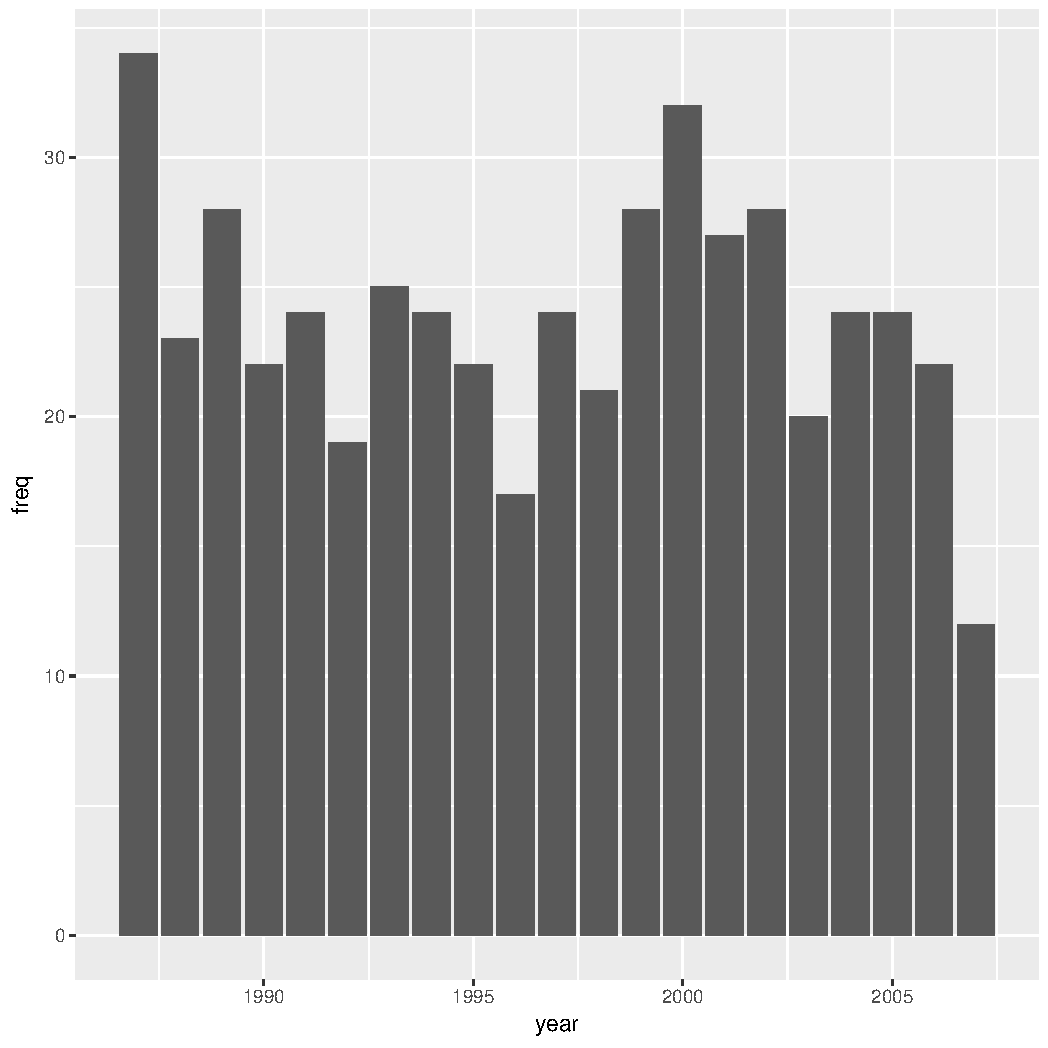
\includegraphics[width=1.0\textwidth]{../result/timeLineYear.pdf}
\caption{timeLineYear}
\label{fig:timeLineYear}
\end{figure}

\section{新闻相似度计算}
通过tm中函数DocumentTermMatrix(corpus)得到文档-词语矩阵,其中每一行就是新闻的BoW向量表示。
相关函数getWordMatrix()。
\subsection{计算新闻之间的余弦相似度矩阵}
用BoW向量计算新闻之间的余弦相似度,时间复杂度$O(mn^2)$,m为向量长度(总词数),n为文档数。这一步
非常耗时,主要原因在于m太大。因此在扩展分析部分尝试对此进行改进。主要函数getSimilarityMat(),
在process.R中,使用公式
\begin{eqnarray*}
  cos\_sim(\mathbf{x},\mathbf{y})=
  \frac{\mathbf{x}\cdot \mathbf{y}}
  {\lVert \mathbf{x} \rVert \lVert \mathbf{y} \rVert}
\end{eqnarray*}
计算余弦相似度矩阵的上三角部分,由对称性下三角可得,对角线置为1。
结果在result/similarityMatrix.csv。
\subsection{计算类别内新闻之间的平均相似度}
有了相似度矩阵和类别标签,就能计算类别$i$和类别$j$新闻之间的平均相似度。形式化表示如下:
\begin{eqnarray*}
  avg\_sim(i,j) = \left\{
                  \begin{aligned}
                  &mean_{ii\in i,jj\in j}(sim(ii,jj)) &  & j\neq i \\
                  &mean_{ii\in i,jj\in j,ii\neq jj}(sim(ii,jj)) &  & j=i 
                  \end{aligned}
                  \right.
\end{eqnarray*}
不同类别间的相似度就是两个类别所有新闻pair的相似度取平均。类别内新闻相似度是除了相同新闻间的相似度
取平均。getCrossDistance()计算得到类别间平均相似度矩阵,
其中对角元素就是类别内新闻之间的平均相似度。结果见
result/innerDistance.csv,使用drawInnerDistance()作图,见\ref{fig:innerDistance}。
其中automobile为1是因为只有一篇相关新闻。

\begin{figure}[htbp]
\centering
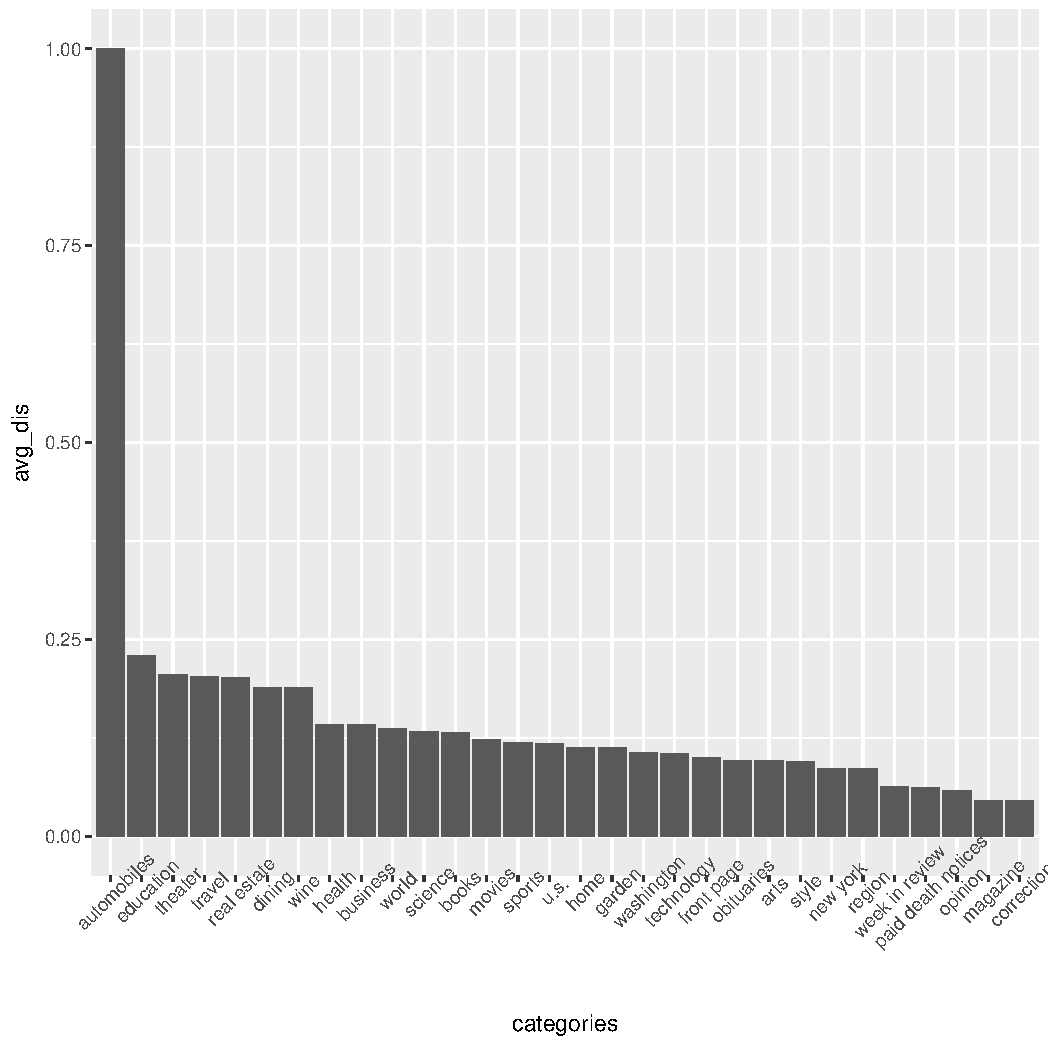
\includegraphics[width=1.0\textwidth]{../result/innerDistance.pdf}
\caption{innerDistance}
\label{fig:innerDistance}
\end{figure}

\subsection{计算两个类别的新闻之间的平均相似度}
类别间平均相似度矩阵见result/relativityMatrix.csv。queryDistance()可用于查询两个类别新闻
之间的平均相似度。

\section{扩展分析}
针对BoW向量太长的问题,想借助SVD进行降维处理。在drawSVDrepr()中,将文档-词语矩阵通过SVD分解,
得到文档语义相关矩阵datau和词项语义相关矩阵datav。取矩阵的前两维,即是对恢复原矩阵帮助最大,
保留信息最多的两维进行作图分析,降维后文档的分布如\ref{fig:doc},词语的分布如\ref{fig:word}。
很难从中获得一些可解释的信息,猜测是降维降得太厉害了,二维的投影很难表现原来成百上千维的内容。

\begin{figure}[htbp]
\centering
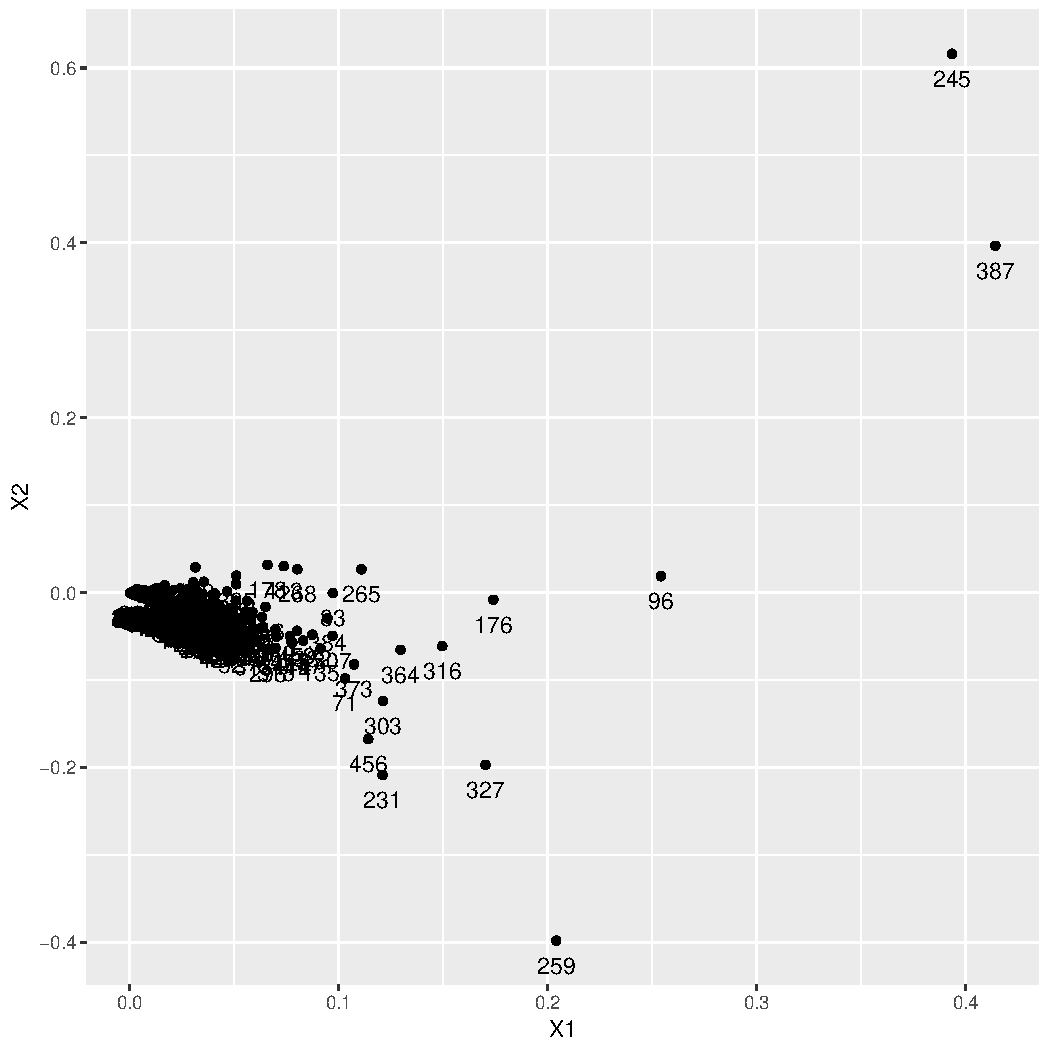
\includegraphics[width=1.0\textwidth]{../result/doc.pdf}
\caption{doc repr}
\label{fig:doc}
\end{figure}

\begin{figure}[htbp]
\centering
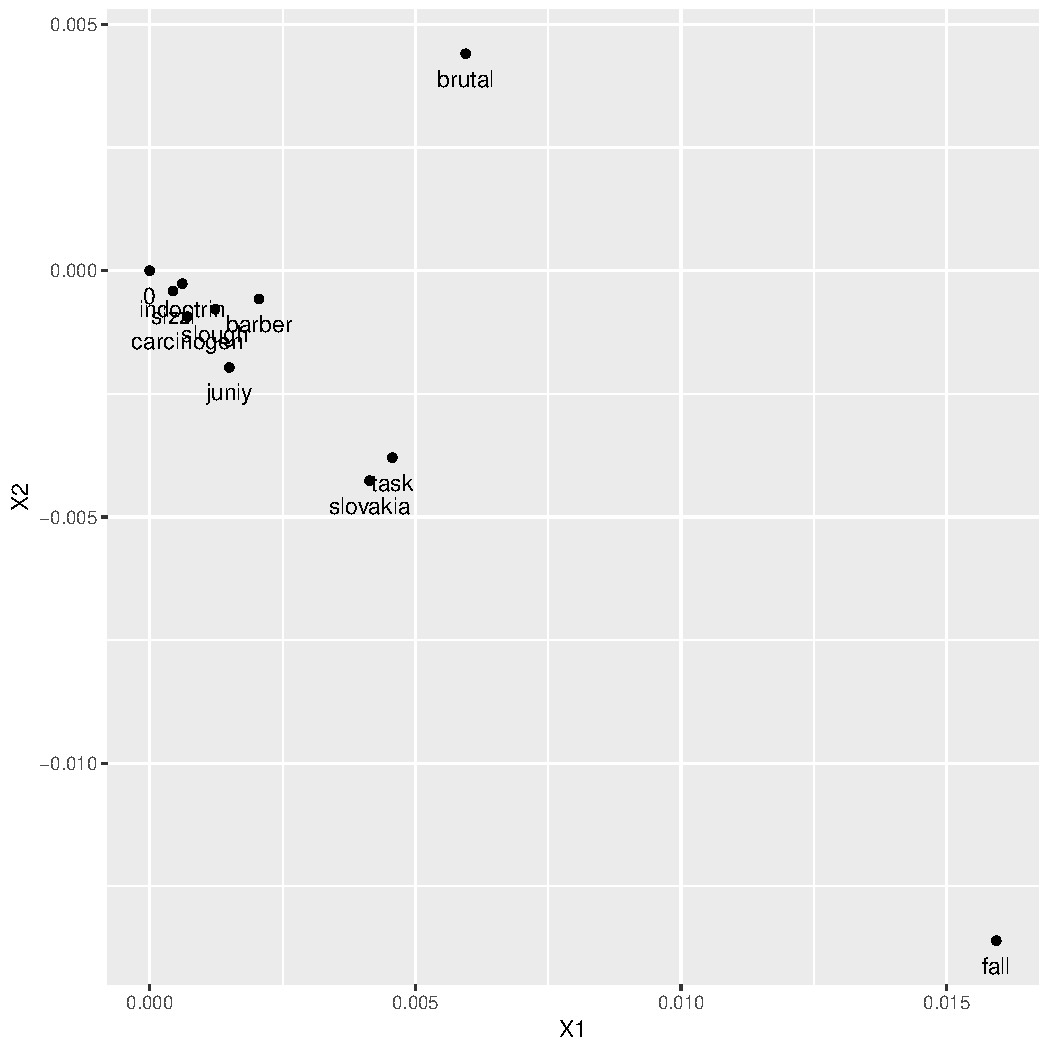
\includegraphics[width=1.0\textwidth]{../result/word.pdf}
\caption{word repr}
\label{fig:word}
\end{figure}

\end{document}  

